\documentclass[a4paper,10pt]{book}
\usepackage[utf8]{inputenc}

\renewcommand{\familydefault}{\sfdefault}

\usepackage{textcomp}
\usepackage{listings}
\usepackage{enumitem}
\usepackage{xcolor}
\usepackage{environ}
\usepackage{pdfpages}
\usepackage{amsmath}

\newcommand{\PPODESUITE}{PPODE SUITE}
\newcommand{\PPODE}{\emph{PPODE}}
\newcommand{\MATLAB}{MATLAB}
\newcommand{\MSDOS}{Windows}
\newcommand{\MATHWORKS}{MathWorks}
\newcommand{\UBUNTU}{Ubuntu}
\newcommand{\nix}{\textborn nix}
\newcommand{\Fortran}{Fortran}

\newcommand{\shellcmd}[1]{\\\indent\indent\texttt{\footnotesize \$ #1}\\}
\newcommand{\matlabcmd}[1]{\\\indent\texttt{\footnotesize >> #1}\\}
\newcommand{\matlabcmdinline}[1]{\textacutedbl\texttt{\footnotesize#1}\textgravedbl}
\newcommand{\sourceword}[1]{\texttt{\footnotesize#1}}
\newcommand{\ph}[1]{\textcolor{gray}{\textlangle #1\textrangle}}
\newcommand{\filepath}[1]{{\footnotesize\textacutedbl #1\textacutedbl}}
\newcommand{\hyperlink}[1]{\emph{\footnotesize#1}}

\lstdefinestyle{fortrancode}{
  basicstyle=\fontsize{7pt}{1em}\ttfamily,
  frame=tb,
  backgroundcolor=\color[rgb]{0.99,0.99,0.99},
  escapechar=\%
}

\newcommand{\pchapter}[1]{\chapter{#1}}
\newcommand{\psection}[1]{\section{#1}}
\newcommand{\psubsection}[1]{\subsection{#1}}

\def \figPath {./graphics/}

\title{\PPODESUITE\\Manual}
\author{Pascal A. Pieters}
\date{March 2014}

\begin{document}

\frontmatter
\maketitle
\tableofcontents

\mainmatter
\chapter[Introduction]{Introduction}
The \PPODESUITE aims to bring ordinary differential equation (ODE) solvers to \MATLAB that - in a lot of cases - will increase the performance with respect to the default ODE solvers provided \MATLAB. The default \MATLAB ODE solvers use the \MATLAB language to define the ODE system, which allows access to the wide variety of \MATLAB functions and toolboxes. However, since \MATLAB is a scripting language, the execution of \MATLAB code requires an extra interpretation step at every execution compared to languages like C/C++ and \Fortran, which require a translation step only once (Figure \ref{fig:InterpretationVSCompilation}).
\begin{figure}[hb]
 \centering
 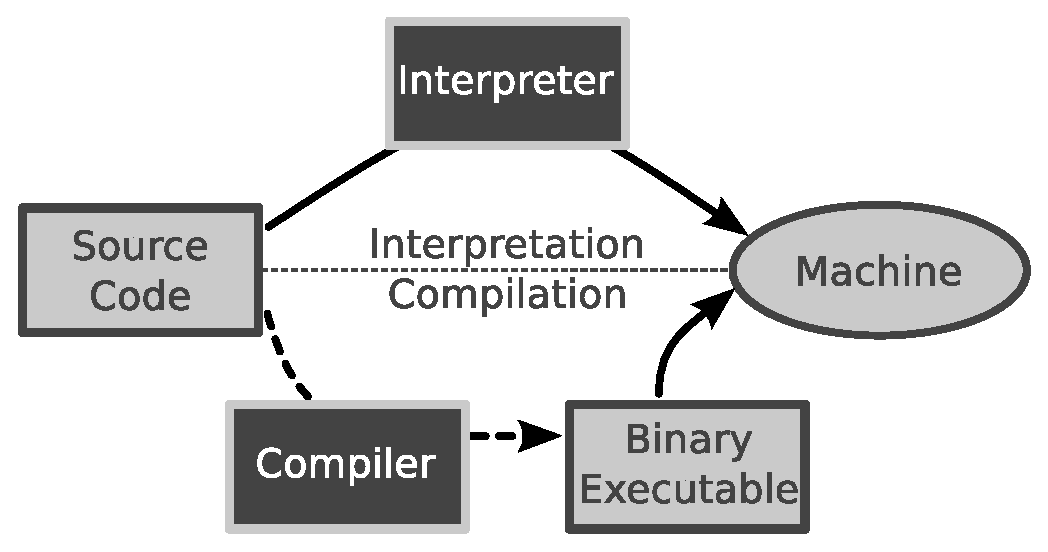
\includegraphics[width=0.6\textwidth]{./graphics/interpreter-vs-compiler.eps}
 \caption{Schematic overview of the difference between translation/compilation and interpretation. Dotted arrows represent translation steps, whereas solid arrows represent execution steps. Interpretation generates has a delay every execution, compilation only requires a (slow) execution step once. This compilation step generates a binary machine-readable file, which can be executed almost directly on the hardware layer of a computer.}
 \label{fig:InterpretationVSCompilation}
\end{figure}

Considering the differences between compilation and interpretation, various cases can be identified where compilation would be preferable over interpretation. In general, compilation is superior when the number of executions desired eliminates the overhead of the compilation procedure (e.g. data fitting). This holds as long as no \MATLAB specific functions or toolboxes are being used, which is mostly not the case for ODE systems.

%TODO: Reference to PUAMAT/CVODE Parser

Furthermore, there is a more specific problem with the build-in \MATLAB solvers, namely that not for every specific situation the most suitable solver is available. For example, large systems of sparsely interlinked differential equations (e.g. Equation \ref{eq:BandedExample}) become time consuming to solve using \MATLAB.
\begin{equation} \label{eq:BandedExample}
  \frac{d\mathbf{F}}{dt} =
  \begin{pmatrix}
   -\alpha_1 & \alpha_2 & 0 & \cdots & \cdots & 0 \\
   \alpha_1 & -\alpha_2 & \alpha_3 & \ddots & \ddots & \vdots \\
   0 & \alpha_2 & -\alpha_3 & \alpha_4  & \ddots & \vdots \\
   \vdots & \ddots & \ddots & \ddots & \ddots & \vdots  \\
   0 & \cdots & \cdots & \cdots & \alpha_{n-1} & -\alpha_{n} \\
  \end{pmatrix}
  \mathbf{F}
\end{equation}
However, suitable solutions for these problems exist. The fast increase of time it takes to solve the system is caused by an exponentially increasing Jacobian matrix. The Jacobian matrix is used by stiff solvers and defined as shown in Equation \ref{eq:Jacobian}.
\begin{equation} \label{eq:Jacobian}
  J_{m,n} =
  \begin{pmatrix}
   \frac{\partial F_1}{\partial x_1} & \cdots & \frac{\partial F_1}{\partial x_n} \\
   \vdots & \ddots & \vdots  \\
   \frac{\partial F_m}{\partial x_1} & \cdots & \frac{\partial F_m}{\partial x_n}
  \end{pmatrix}
\end{equation}
Where $F$ represents the system of ODEs. In the case of an ODE system, $m$ and $n$ are both equal to the number of equations ($N$). This means that the number of elements of the Jacobian matrix increases exponentially, resulting in the following behaviour:
\begin{equation}
 i_{Jac} = N^2 \Rightarrow
 t_{Jac,op} = \Omega(N^2)
\end{equation}
Where $i_{Jac}$ is the number of elements in the Jacobian matrix and $t_{Jac,op}$ the time a typical operation on the Jacobian matrix takes.

In the specific case of Equation \ref{eq:BandedExample}, the Jacobian matrix is a band matrix, which enables specialized matrix handling methods for the Jacobian matrix, which only make $t_{Jac,op}$ increase linearly.

A more general method is the use of a sparse implementation of the Jacobian matrix. This allows elements of the Jacobian matrix not in the center band to be non-zero, in contrast to band matrix implementations. This suite was created to enable \MATLAB to call this type of ODE solvers, following the need to solve large nucleation-elongation ODE systems. These system make use of a cut-off to limit the number of equations, since the exact system consists of an infinite amount of equations. To facilitate the use of a cut-off, the number of equations was left variable and can vary between function calls, without the need to recompile the code.

Next to these specific "sparse Jacobian" solvers, a wide variety of other solvers - all written in the \Fortran programming language - is available through this suite, for an overview see Chapter \ref{ch:Solvers}. The suite consist of the following tools:
\begin{description}
 \item[PPODE\_init] builds the ODE solver libraries and in principle only has to be executed once. See Chapter \ref{ch:Installation}.
 \item[PPODE\_addPaths] loads paths of the \PPODESUITE into the \MATLAB path variable. To access the \PPODESUITE, this function has to be executed. See Chapter \ref{ch:Installation}.
 \item[PPODE\_parser] parses a \MATLAB ODE function to \Fortran. The use of this function eliminates the need for knowledge about the \Fortran programming language. See Chapter \ref{ch:Usage}.
 \item[PPODE\_build] builds the \Fortran function generated by PPODE\_parser. Of course, one can also manually provide a \Fortran function. See Chapter \ref{ch:Usage}.
\end{description}

\chapter[Installation]{Installation}
The \PPODESUITE package depends on:
\begin{description}
  \item[\MATLAB] Tested on \MATLAB version R2013b (8.2) 64-bit.
  \item[gfortran and GCC] Tested on version 4.8.1 64-bit.
\end{description}

\section[\nix]{Linux and other Unix variants}
\begin{enumerate}
 \item Meet the software requirements by installing \MATLAB and the GCC package. \MATLAB download and installation instructions can be found on the \MATHWORKS website. The gfortran/GCC package can be obtained from the \nix distribution repository through the distribution package manager. Using \UBUNTU for example:
 \shellcmd{sudo apt-get install gfortran gcc}
\end{enumerate}

\section[Windows]{\MSDOS}
\textbf{Currently, running the \PPODESUITE on \MSDOS is not supported nor tested.}
\begin{enumerate}
 \item Running the \PPODESUITE on \MSDOS would require installing a combination of GCC/Cygwin and gnumex (\hyperlink{http://gnumex.sourceforge.net/}) or the Intel Visual Fortran Composer. To check which versions are supported by \MATLAB, check \hyperlink{http://www.mathworks.nl/support/compilers/R2013b/} substituting R2013b with the right version number.
\end{enumerate}

\section{General}
\begin{enumerate}[resume]
 \item Download and extract the \PPODESUITE package.
 \item Open matlab and navigate to the extracted \PPODESUITE folder. Add the \PPODE paths to the matlab path variable.
 \matlabcmd{PPODE\_addPaths}
 \item Now the libraries of the different solvers can be build. In order to do so, execute the following command;
 \matlabcmd{PPODE\_init}
 The options 'Debug' can be used to build the libraries with debugging symbols.
 \matlabcmd{PPODE\_init('Debug', 1)}
 For more information, type \matlabcmdinline{help PPODE\_init} in the \MATLAB command window.
\end{enumerate}

\chapter{Usage} \label{ch:Usage}
The ODE solvers need an ODE system to be provided as a \Fortran subroutine (function), this can be done either manually or using the parser provided by the \PPODESUITE. Both options are described in the next two sections.
\section{Manual ODE Function}
\subsection{Introduction}
The ODE function of the problem should be written in \Fortran 95. Here are some main \Fortran peculiarities to consider when writing \Fortran code.
\begin{description}
 \item[Line Formatting] The maximum line width is 72 characters. The first character is used to indicate whether the line is a comment line. The second to fifth character are used to indicate labels. The $6^{th}$ character is used to indicate the continuation of the previous line.
 \begin{lstlisting}[style=fortrancode,caption=Syntax Example]
c         1         2         3         4         5         6         7
c23456789012345678901234567890123456789012345678901234567890123456789012

! Comments should be introduced by either a 'c' or a '!'.
      if (answer .gt. 42) go to 4242
 4242 ydot(s) = y(1) * (kp * y(s - 1) - gp * y(s)) + gm * y(s + 1) +
     + km * y(s)
 \end{lstlisting}
 \item[For Loops] For loops are written using the \sourceword{do} statement. They should be written in the form \sourceword{do \ph{label} \ph{var}=\ph{start}, \ph{stop}[, \ph{step}]}. The label should refer to a \sourceword{continue} statement at the end of the loop.
  \begin{lstlisting}[style=fortrancode,caption=Do-Loop]
      a = 0
      do 42 i=1, 20
        a = a + 1
   42 continue
! a has the value 20 here.
 \end{lstlisting}
 \item[Case Sensitivity] The \Fortran language is not case sensitive.
 \item[Vectors] Vectors indexing starts at 0, just like in \MATLAB.
\end{description}

\subsection{Template}
The \Fortran subroutine that defines the ODE system should have the following arguments:
\begin{description}
 \item[neq] \emph{input} Number of equations.
 \item[t] \emph{input} The current time point.
 \item[y] \emph{input} The current value of all states. The length of this vector is equal to \sourceword{neq}.
 \item[np] \emph{input} Number of parameters.
 \item[p] \emph{input} Vector of the values of all parameters.
 \item[ydot] \emph{output} This is a vector of length \sourceword{neq} to which all derivatives of the states should be written.
\end{description}

\lstinputlisting[style=fortrancode,caption=ODE Template]{ODETemplate.F}

Examples can be found in the \filepath{\ph{\PPODESUITE Source}/examples} folder.

\section{Parser} \label{sec:Parser}
\PPODESUITE can translate a \MATLAB function to \Fortran. The function that executes this procedure is PPODE\_translate. The parser is created using a combination of lex and yacc/bison. The parser interprets the the \MATLAB code and creates a tree structure out of it. This tree structure is then used to create the \Fortran code. This provides more flexibility and better interpretation than more direct forms of translation. An additional benefit is that the structure can be used to determine the Jacobian of the function.

\subsection{Restrictions and Pitfalls}
The \MATLAB ODE function should have the following structure:
\matlabcmd{\ph{dx} = func( \ph{t}, \ph{x}, \ph{par}, \ph{neq}, \ph{np} )}
Where \ph{t} is the independent variable, \ph{x} the dependent variable(s) and \ph{par} the parameter values. The last two arguments are optional and represent the number of equations (\ph{neq}) and number of parameters (\ph{np}).

If the number of equations is not fixed, it should always depend on \ph{neq}. If you would for example use $\gamma$ as a parameter, which would per definition result in $2\cdot\gamma$ equations, define $\gamma = {neq \over 2}$ in your code, instead of passing $\gamma$ as a parameter.

One of \MATLAB's main benefits is the ease of using vectors and matrices. Not all of this functionality can easily be ported to \Fortran, therefore there are some restrictions to consider when using vectors. First of all, matrices are (currently) not supported, only 1-dimensional datatypes are supported, i.e. vectors. Moreover, \MATLAB supports dynamic vectors (vectors that can change size during exection). This could be implemented in \Fortran, but it was chosen not to since almost all code that is written using dynamic vectors can also be written using static vectors, which in most cases is much faster. So make sure the size of vectors does not change in the ODE function and \textbf{all vectors are initialized using the \matlabcmdinline{zeros} function.}

For example, the following code will not be parsed correctly and is slow and a bad coding practice in general:
\matlabcmd{dx = []; dx = [dx da]; dx = [dx da];}
Here, the vector \texttt{dx} is initialized as an empty vector and changes size twice afterwards. Better code, that can be translated to \Fortran is the following:
\matlabcmd{i = length(da); dx = zeros(2*i, 1); dx(1:i) = da; dx((i+1):(2*i)) = da;}

Furtermore, bear in mind that \MATLAB has a lot of specific functions, that will are not implemented in \Fortran or the parser and will therefore not work.

\section[Building]{Building the MEX Function}
The \MATLAB function \sourceword{PPODE\_build}, included in the \PPODESUITE, can be used to build the ODE \Fortran file against the right solver libraries. First of all, make sure the \PPODESUITE paths are added to the \MATLAB path variable.
\matlabcmd{PPODE\_addPaths}
And the libraries are build.
\matlabcmd{PPODE\_init}
Now the function \sourceword{PPODE\_build} can be used. Extensive help can of course be acquired using \matlabcmdinline{help PPODE\_build}. The simplest usage of the function is the following:
\matlabcmd{PPODE\_build('odeproblem.F', 'odeproblem\_stiffsolver')}
This command will generate a MEX file named 'odeproblem\_stiffsolver' of the problem defined by 'odeproblem.F', using the default (stiff) solver. The correct file extension is automatically added to the MEX file, so do not supply an extension for the second function argument.

The first two mandatory arguments, extra options can be specified. This is done by first giving the option name and then the value. For example, if the problem is not stiff and one would like verbose output, a non-stiff solver should be specified and the verbose mode should be enabled:
\matlabcmd{PPODE\_build('odeproblem.F', 'odeproblem\_stiffsolver', ...\\\indent\indent'Solver', 'Non-Stiff', 'Verbose', 1)}
Note that both the option name and value are case insensitive.

\subsection{Sparse Jacobian Matrix}
When using the solver that uses a sparse matrix implementation for the Jacobian matrix, the number of non-zero values of the Jacobian matrix should be supplied. There are two options to tackle this problem.

The first and default option needs an analytical Jacobian to be specified. The generated function will evaluate the Jacobian two times to determine the number of non-zero elements. This option can be selected by setting 'INPUTNNZ' to zero.

The second option is to manually provide a number of non-zero elements. This option can be selected by settting 'INPUTNNZ' to one. When this option is set, the generated function will require the first argument to be a 2x1 vector consisting of first the number of equations, and second the number of non-zero elements.

In order to determine the number of non-zero elements of the Jacobian matrix, consider the definition of this matrix:
\begin{equation}
  J_{m,n} =
  \begin{pmatrix}
   \frac{\partial F_1}{\partial x_1} & \cdots & \frac{\partial F_1}{\partial x_n} \\
   \vdots & \ddots & \vdots  \\
   \frac{\partial F_m}{\partial x_1} & \cdots & \frac{\partial F_m}{\partial x_n}
  \end{pmatrix}
\end{equation}
In the case of an ODE system, $m$ and $n$ are both equal to the number of equations. $F$ represents the system of ODEs.
The number of nonzero elements can also be determined using trial and error. By just trying some values for \sourceword{nnz}, the error messages might give away the correlation between \sourceword{nnz} and the parameter and number of equations (this does not work with LSODES).

\section[Execution]{Executing the MEX Function}
The MEX function generated by the PPODE build function can be called as follows:
\matlabcmd{[\ph{t}, \ph{y}] = \ph{F}(\ph{neq}, \ph{abstol}, \ph{reltol}, \ph{times}, \ph{par}, \ph{y0})}
Where \ph{F} is the name of the MEX function, \ph{neq} is the number of equations, \ph{abstol} and ph{reltol} are the absolute and relative tolerances respectively, \ph{times} is a vector of time points at which output is desired, \ph{par} is a vector of parameter values and \ph{y0} is a vector of the initial values of the states. The function returns the vector \ph{t} with the time points at which the values of the states are calculated. The matrix \ph{y} contains the values of all states at the time points specified by \ph{t}.

\pchapter{Solvers} \label{ch:Solvers}
\psection{Introduction}
The solver for the ODE problem can be specified using the 'Solver' option of the \sourceword{PPODE\_build} function:
\matlabcmd{PPODE\_build(\ph{source}, \ph{target}, 'Solver', \ph{solver})}
Valid options for \ph{solver} are:
\begin{description}
 \item['Stiff' (or 'BDF')] The BDF based solver of the LSODE package. \emph{See \ref{subsec:LSODEBDF}}.
 \item['Stiff2' (or 'VODE')] The BDF based solver of the VODE package. \emph{See \ref{subsec:VODEBDF}}.
 \item['MEBDFSO' (or 'MEBDFSparse')] The modified extended BDF based solver using a sparse Jacobian matrix. \emph{See \ref{subsec:MEBDFSO}}.
 \item['LSODES' (or 'BDFSparse')] The BDF based solver using a sparse Jacobian matrix. \emph{See \ref{subsec:LSODES}}.
 \item['Non-Stiff' (or 'Adams-Moulton')] The Adams-Moulton based solver of the LSODE package. \emph{See \ref{subsec:LSODEAM}}.
 \item['Non-Stiff2' (or 'VODEAM')] The Adams-Moulton based solver of the VODE package. \emph{See \ref{subsec:VODEAM}}.
 \item['RK23', 'RK45', 'RK78'] The Runge-Kutta based solvers of the RKSUITE package. \emph{See \ref{subsec:RKSUITE}}.
 \item['Switching' (or 'LSODA')] The solver that switches between the non-stiff Adams-Moulton based solver and the stiff BDF based solver of the LSODE package. \emph{See \ref{subsec:LSODA}}.
\end{description}

If you do not know which solver to choose, but you already know which \MATLAB~solver performs best, table \ref{tab:MATLABToPPODE} might be helpfull.
\begin{table}
\begin{tabular}{ | l || l | p{5cm} | } \hline
 \textbf{\MATLAB} & \textbf{Equivalent} & \textbf{Probably Also Suitable} \\
 \hline
 \hline
 ode45 & 'RK45' & 'RK78', 'Non-Stiff', 'Non-Stiff2' \\ \hline
 ode23 & 'RK23' & 'RK45', 'Non-Stiff', 'Non-Stiff2' \\ \hline
 ode113 & 'Non-Stiff', 'Non-Stiff2' & 'RK45' \\
 \hline
 \hline
 ode15s & 'Stiff', 'Stiff2' & 'Switching' (partially stiff problems), 'MEBDFSO' (large number of states that are not very interdependent) \\ \hline
 ode23s & - & 'Stiff', 'Stiff2', 'Switching', 'MEBDFSO' \\ \hline
 ode23t & - & 'Switching', 'Stiff', 'Stiff2', 'MEBDFSO' \\ \hline
 ode23tb & - & 'Switching', 'Stiff', 'Stiff2', 'RK45', 'RK23', 'MEBDFSO' \\ \hline
\end{tabular} 
\caption{Solver selection helper.\label{tab:MATLABToPPODE}}
\end{table}

\psection{Stiff}
\psubsection{BDF}
\label{subsec:LSODEBDF}
The Backward Differential Formulas based method uses the BDF implementation that ODEPACK supplies. The order of these formulae can range between 1 and 5 and can be limited by setting the 'MaxOrder' option when building the ODE system.

\subsubsection{Credits}
Credits for the ODEPACK package obtained from (\hyperlink{http://www.netlib.org/}).

\vspace{0.5cm}
\begin{tabular}{ l l }
 \textbf{Author}      & Alan C. Hindmarsh \\
 \textbf{Institution} & Center for Applied Scientific Computing, L-561 \\
                      & Lawrence Livermore National Laboratory \\
                      & Livermore, CA 94551 \\
                      & United States of America \\
\end{tabular}
\psubsection{Modified Extended BDF using Sparse Jacobian}
\label{subsec:MEBDFSO}
The Modified Extended Backward Differential Formulae based method uses the BDF implementation that MEBDFSO supplies. The order of these formulas can range between 1 and 5 and can be limited by setting the 'MaxOrder' option when building the ODE system.

\subsubsection{Credits}
Credits for the MEBDFSO package obtained from (\hyperlink{http://www.netlib.org/}).

\vspace{0.5cm}
\begin{tabular}{ l l }
 \textbf{Authors}     & T.J. Abdulla \\
                      & J.R. Cash \\
 \textbf{Institution} & Department of Mathematics \\
                      & Imperial College \\
                      & London SW7 2AZ \\
                      & England \\
 \textbf{Contact}     & t.abdulla@ic.ac.uk \\
                      & j.cash@ic.ac.uk \\
\end{tabular}

\psection{Non-Stiff}
\psubsection{Adams-Moulton Methods}
\label{subsec:LSODEAM}
The Adams-Moulton method based solver uses the Adams-Moulton implementation that ODEPACK supplies. The order of these formulae can range between 1 and 12 and can be limited by setting the 'MaxOrder' option when building the ODE system.
\subsubsection{Credits}
Credits for the ODEPACK package obtained from (\hyperlink{http://www.netlib.org/}).

\vspace{0.5cm}
\begin{tabular}{ l l }
 \textbf{Author}      & Alan C. Hindmarsh \\
 \textbf{Institution} & Center for Applied Scientific Computing, L-561 \\
                      & Lawrence Livermore National Laboratory \\
                      & Livermore, CA 94551 \\
                      & United States of America \\
\end{tabular}

\psubsection{Runge-Kutta Methods}
\label{subsec:RKSUITE}
The Runga-Kutta methods based solver uses the RKSUITE package. Three Runge-Kutta pairs are available: 2-3, 4-5 and 7-8. Use higher orders in combination with smaller tolerances.
\subsubsection{Credits}
Credits for the RKSUITE package obtained from (\hyperlink{http://www.netlib.org/}).

\vspace{0.5cm}
\begin{tabular}{ l l }
 \textbf{Author}      & R.W. Brankin \\
 \textbf{Institution} & Numerical Algorithms Group Ltd. \\
                      & Wilkinson House \\
                      & Jordan Hill Road \\
                      & Oxford OX2 8DR \\
                      & United Kingdom \\
 \textbf{Contact}     & richard@nag.co.uk \\
                      & na.brankin@na-net.ornl.gov \\
 \textbf{Authors}     & I. Gladwell \\
                      & L.F. Shampine \\
 \textbf{Institution} & Department of Mathematics \\
                      & Southern Methodist University \\
                      & Dallas, Texas 75275 \\
                      & United States of America \\
 \textbf{Contact}     & h5nr1001@vm.cis.smu.edu \\
\end{tabular}
\psection{Mixed}
\psubsection{Switching between BDF and Adams-Moulton Methods}
\label{subsec:LSODA}
The switching method uses the LSODA subroutine that the ODEPACK package supplies. This method automatically switches between the BDF based stiff solver (order 1-5) and the Adams-Moulton methods based non-stiff solver (order 1-12).

\subsubsection{Credits}
Credits for the ODEPACK package obtained from (\hyperlink{http://www.netlib.org/}) and the LSODA subroutine in particular.

\vspace{0.5cm}
\begin{tabular}{ l l }
 \textbf{Author}      & Alan C. Hindmarsh \\
 \textbf{Institution} & Center for Applied Scientific Computing, L-561 \\
                      & Lawrence Livermore National Laboratory \\
                      & Livermore, CA 94551 \\
                      & United States of America \\
 \textbf{Author}      & Linda R. Petzold \\
 \textbf{Institution} & Univ. of California at Santa Barbara \\
                      & Dept. of Computer Science \\
                      & Santa Barbara, CA 93106 \\
                      & United States of America \\
\end{tabular}


\end{document}
